\setcounter{secnumdepth}{1}
\section{Einführung}
Diese Bachelorarbeit behandelt die Ausführung und Verarbeitung von asynchronen Prozessen in der Programmierung speziell in der Sprache Typescript.\\
Zielgruppe dieser Arbeit sind Personen, die Grundkenntnisse in der Sprache Javascript/Typescript vorweisen können.
Sollte man von der Skriptsprache Typescript noch nicht/kaum etwas gehört haben, sollte vor dem Lesen dieser Arbeit die offizielle Dokumentation von Microsoft durchgegangen werden.

\begin{center}
\url{https://www.typescriptlang.org/docs/home.html} 
\end{center}

In dieser Arbeit wird nur oberflächlich auf die Unterschiede der beiden Sprachen eingegangen. Des Weiteren sollte man von den Kernkonzepten der Promises und Observables schon mal gehört haben, da diese in der Arbeit gegenübergestellt werden.

\subsection{Typescript}
Typescript. Bereits der Name sagt schon was diese Sprache ausmacht. Sie \textit{(\glqq{}Type\grqq{} zu deutsch: Typ)} ist eine typisierte Form der Skriptsprache Javascript. In Typescript ist es Standard, jede Variable, Funktion und Funktionsparameter im Vorfeld zu typisieren. Mit dem Typescript Compiler werden Dateien mit dem Suffix *.ts in *.js überführt.

\subsubsection{Beispiel}

\begin{figure}[h!]
\begin{lstlisting}
class Greeter {
    greeting: string;
    constructor (message: string) {
        this.greeting = message;
    }
    greet() {
        return "Hello, " + this.greeting;
    }
}  
\end{lstlisting}
\caption{Typescript Klasse \cite{typescript-example}}
\end{figure}

Im oberen Code-Schnipsel wurden die variablen und die Klassenmethoden nach Typescript-Standard deklariert. Diese Typen werden beim übersetzen in Javascript ignoriert. Der Kompiler einer Entwicklungsumgebung prüft dann, ob beim übergeben eines Parameters in den Konstruktor ein numerischer oder Boolean-Wert eingesetzt wird. Dies wird dann als ein Fehler erkannt. Der Kompiler übersetzt auch nicht direkt deklarierte Typen. Wie in diesem Fall wird erkannt, dass die Methode greet() einen String-Wert zurückgibt.

\begin{figure}[t]
\begin{lstlisting}
var Greeter = (function () {
    function Greeter(message) {
        this.greeting = message;
    }
    Greeter.prototype.greet = function () {
        return "Hello, " + this.greeting;
    };
    return Greeter;
})(); 
\end{lstlisting}
\caption{Überführung in Javascript \cite{typescript-example}}
\end{figure}
In der vom Kompiler auf Javascript übersetzten Version werden die erstellten Klassen und Typen vollständig eliminiert. Was verbleibt ist die Übersetzung der Klassen-Methode greet() und des Konstruktors. Sowohl Klassen als auch Interfaces werden in Javascript nicht genutzt.

\subsubsection{Kompiler}

In einer tsconfig.json Datei können die Kompiler-Optionen für Typescript gesetzt werden. Zudem können Root-Dateien definiert und ausgeschlossen werden. Die Auflistung einer tsconfig.json Datei in einem Verzeichnis zeigt, dass das es sich hierbei um das Root-Verzeichnis des Projekts handelt. Ein Beispiel für die Konfiguration einer solchen Datei könnte folgend aussehen: 

\begin{figure}[h!]
\begin{lstlisting}
{
    "compilerOptions": {
        "module": "system",
        "noImplicitAny": true,
        "removeComments": true,
        "preserveConstEnums": true,
        "outFile": "../../built/local/tsc.js",
        "sourceMap": true
    },
    "include": [
        "src/**/*"
    ],
    "exclude": [
        "node_modules",
        "**/*.spec.ts"
    ]
}  
\end{lstlisting}
\caption{tsconfig.json \cite{tsconfig}}
\end{figure}
Hier kann z.B. mit der Regel 
\glqq noImplicitAny\grqq{} verhindert werden, dass Methoden als auch Parameter und Variablen getypt werden müssen bei ihrer Deklaration. Sind sie nicht getypt: Bedeutet dies für den Kompiler sie sind als any zu deklariert.
Die Konfiguration dieser Datei betrifft Kompilier-Fehler. Fehler zur Laufzeit sind von der Konfiguration ausgeschlossen.\\\\

Da Syntaktisch alles was auf Javascript geschrieben auch valider Typescript Code ist, kann man Typescript als Superset von Javascript bezeichnen.
Demzufolge kann man die Nutzung von  statische Typen, Klassen und Interfaces als Konvention betrachten.

Im Laufe der Zeit findet typescript immer mehr Beliebtheit in Unternehmensprojekten. Entwicklerteams können durch die Typisierung schneller Bugs am Code erkennen und durch den modularen Aufbau, den Typescript ermöglicht, die Organisation und Dokumentation von großen Projekten verbessern. Diese Tendenz wird von der beliebten Entwicklerplattform Stackoverflow untermauert, die laut einer Umfrage welche die beliebtesten Programmiersprachen unter Entwickler sei, folgendes rausgekommen ist:

\begin{figure}[H]
\centering
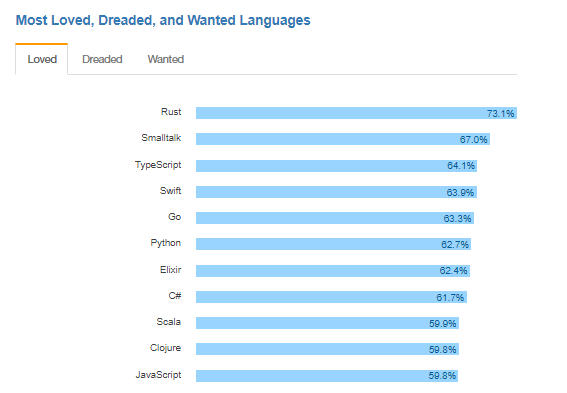
\includegraphics[height=6cm]{stackoverflow-typescript-popularity}
\caption{Prozentualer Anteil der Entwickler die Interesse an neuen Technologien zeigen und weiter mit neuen Technologien arbeiten möchten. Jahr: 2017 \cite{typescript-survey}}
\end{figure}

\begin{enumerate} 
\item Motivation hinter der Bachelorarbeit
\item Was kann man aus dieser Bachelorarbeit "gewinnen"?
\end{enumerate}

\section{Vorbereitung}
\begin{enumerate} 
\item Welches Framework wird verwendet (Wenn überhaupt?) und welche Sprache angewandt?
\item Repo-Referenz
\end{enumerate}

\subsection{Einführung in asynchrone Operationen}
*Source-code Beispiel*